\documentclass[11pt]{article}
\usepackage[margin=0.8in]{geometry}
\usepackage[]{amsfonts, amssymb, amsmath, float, hyperref,fancyheadings, graphicx, derivative}
\pagestyle{fancy}
\lhead{Machine Learning}
\chead{Larry128}
\rhead{COMP4211}
\renewcommand{\footrulewidth}{0.4pt}
\setcounter{tocdepth}{3} % set TOC
\newcommand{\indep}{\perp \!\!\! \perp}

% codeblocksı
\usepackage{listings}
\usepackage{xcolor}
\definecolor{codegreen}{rgb}{0,0.6,0}
\definecolor{codegray}{rgb}{0.5,0.5,0.5}
\definecolor{codepurple}{rgb}{0.58,0,0.82}
\definecolor{backcolour}{rgb}{0.95,0.95,0.92}
\lstdefinestyle{mystyle}{
    backgroundcolor=\color{backcolour},   
    commentstyle=\color{codegreen},
    keywordstyle=\color{magenta},
    numberstyle=\tiny\color{codegray},
    stringstyle=\color{codepurple},
    basicstyle=\ttfamily\footnotesize,
    breakatwhitespace=false,         
    breaklines=true,                 
    captionpos=b,                    
    keepspaces=true,                 
    numbers=left,                    
    numbersep=5pt,                  
    showspaces=false,                
    showstringspaces=false,
    showtabs=false,                  
    tabsize=3
}
\lstset{style=mystyle}
\lstdefinestyle{customc}{
  language=C++,
  % Add other settings here
}

%common math symbols
\newcommand{\R}{\mathbb{R}}
\newcommand{\N}{\mathbb{N}}
\newcommand{\Q}{\mathbb{Q}}
\newcommand{\ddx}{\dfrac{d}{dx}}
\newcommand{\regressf}{$f(\mathbf{x}; \mathbf{w})$ }
\newcommand{\lossf}{$L(\mathbf{w}; S)$ }

% asymptotic notations
\newcommand\BigO[1]{$O($#1$)$}
\newcommand\BigOmega[1]{$\Omega($#1$)$}
\newcommand\BigTheta[1]{$\Theta($#1$)$}
\newcommand\pddx[2]{\frac{\partial{#1}}{\partial{#2}}}

% pgfplots
\usepackage{pgfplots}
\pgfplotsset{compat=1.18, width=8cm}
\usepackage{geometry}
\geometry{
a4paper,
total={170mm,257mm},
left=20mm,
top=20mm,
}
\usepackage{algorithm}
\usepackage{algpseudocode}

\begin{document}
\begin{titlepage}
    \begin{center}
        \vspace*{1cm}
            
        \Huge
        \textbf{COMP4211}
            
        \vspace{0.5cm}
        \LARGE
        Machine Learning
            
        \vspace{1.5cm}
            
        Larry128
            
        \vfill
            
        A summary notes for revision
            
        \vspace{0.8cm}
                
        \Large
        Fall 2024-2025
            
    \end{center}
\end{titlepage}

\tableofcontents
\newpage

\section{Linear Regression}
\subsection{Basic Ideas of Regression}
\begin{enumerate}
\item Given a training set $S = \{(x^{(l)}, y^{(l)})\}_{l=1}^{N}$ of $N$ labelled examples of input-output pairs.
\item A \textbf{Regression Function} \regressf uses $S$ such that the predicted output $f(\mathbf{x^{(l)}}; \mathbf{w})$ for each input $\mathbf{x}^{l}$ such that $f(\mathbf{x}^{(l)}; \mathbf{w}) \approx \mathbf{y}^l$.
\item (multi-output regression) When the output $\mathbf{y}$ is a vector, it's a multi-output regression.
\item We denote the output by $y$ if the output is univariate.
\item The input $\mathbf{x} = (x_1 , \cdots, x_d) ^T$ is $d$-dimensional.
\end{enumerate}

\subsection{Linear Regression Function}
\begin{enumerate}
\item If the regression function is linear, then 
\begin{align*}
f(\mathbf{x}; \mathbf{w}) &= w_{0} + w_1 x_1 + \cdots + w_d x_d\\
&= \begin{bmatrix}
w_0& w_1& \cdots& w_d
\end{bmatrix} \begin{bmatrix}
1\\
x_1\\
\vdots\\
x_d
\end{bmatrix} &= \begin{bmatrix}
1 & x_1& \cdots& x_d
\end{bmatrix} \begin{bmatrix}
w_0\\
w_1\\
\vdots\\
w_d
\end{bmatrix}\\
&= \mathbf{w}^{T} \mathbf{\tilde{x}} &= \mathbf{\tilde{x}}^{T} \mathbf{w}
\end{align*}
\item $w_0$ is the \textit{bias} term which serves as an offset.
\item The learning problem is to find the best $\mathbf{w}$ according to performance measure on $S$.
\end{enumerate}

\subsection{Loss Function}
\begin{enumerate}
\item A common way to learn the parameter $\mathbf{w}$ of \regressf is to define a loss function \lossf
\item The most common loss function is the \textbf{squared loss}
\begin{align*}
L(\mathbf{w}; S) &= \sum_{l=1}^{N} (f(\mathbf{x}^{(l)} ;\mathbf{w})- \mathbf{y}^{(l)})^2\\
&= \sum_{l=1}^{N} (w_0 + w_1 x_1 ^{(l)}+ \cdots + w_d x_d ^{(l)} - y^{(l)})^2
\end{align*}
\item We may also define the loss function by \textbf{mean} rather than the sum $$L(\mathbf{w}; S) = \dfrac{1}{N} \sum_{l=1}^{N} (f(\mathbf{x}^{(l)} ;\mathbf{w})- \mathbf{y}^{(l)})^2$$
\item A special case ($d=1$)\\
Squared loss: $$L(\mathbf{w}; S) = \sum_{l=1}^{N}(w_0 +w_1 x_1 ^{(l)} - y^{(l)})^2$$
We can find the unique optimal solution $\tilde{\mathbf{w}} = \begin{bmatrix}
w_0\\w_1
\end{bmatrix}$ that minimizes \lossf using the method of least squares.\\
First, we take the derivatives of \lossf with respect to $w_0$ and $w_1$ and set them to $0$.
\begin{align*}
\pddx{L}{w_0} &= 2\sum_{l=1}^{N} (w_0 +w_1 x_1 ^{(l)} - y^{(l)}) =0  \iff \sum_{l=1}^{N}(w_0 +w_1 x_1 ^{(l)}) = \sum_{l=1}^{N} y^{(l)} \iff N w_0 + \sum_{l=1}^{N} w_1 x_1 ^{(l)} = \sum_{l=1}^{N} y^{(l)}\\
\pddx{L}{w_1} &= 2\sum_{l=1}^{N} (w_0 +w_1 x_1 ^{(l)} - y^{(l)})x_1 ^{(l)}=0 \iff w_0 \sum_{l=1}^{N} x_1 ^{(l)} + w_1 \sum_{l=1}^{N} (x_{1}^{(l)})^2 = \sum_{l=1}^{N}x_1 ^{(l)} y^{(l)}
\end{align*}
Then, we have a system of linear equations of two unknown $w_0$, $w_1$. We can write it in matrix form.
\begin{align*}
\mathbf{A} \mathbf{w} = \begin{bmatrix}
N &\sum_{l} x_{1} ^{l}\\
\sum_{l} x_{1} ^{l} &\sum_{l} (x_{1} ^{l})^2
\end{bmatrix} \begin{bmatrix}
w_0\\w_1
\end{bmatrix} = \begin{bmatrix}
\sum_{l} y^{(l)}\\ \sum_{l} x_1 ^{(l)} y^{(l)}
\end{bmatrix} = \mathbf{b}
\end{align*}
Assuming $\mathbf{A}$ is invertible, the least squares estimate is $$\tilde{\mathbf{w}} = \mathbf{A}^{-1} \mathbf{b}$$

\item General case ($d \geq 1$)
\begin{enumerate}
\item (First approach) We express the input and output of $N$ examples as follows
\begin{align*}
\mathbf{X} = \begin{bmatrix}
1& x_1 ^{l}&\cdots & x_{d}^{1}\\
1& x_1 ^{2}&\cdots & x_{d}^{2}\\
\vdots\\
1& x_1 ^{N}&\cdots & x_{d}^{N}
\end{bmatrix}, &&\mathbf{y} = \begin{bmatrix}
y^{(1)}\\
y^{(2)}\\
\vdots\\
y^{(N)}
\end{bmatrix}
\end{align*}
Then we can express the matrix form as follows (proof skipped)
$$\mathbf{A w = X^T X w = X^T y = b}$$
Therefore, the least squares estimate is $$\tilde{\mathbf{w}} = \mathbf{(X^T X)^{-1} X^T y}$$, assuming $\mathbf{X^T X}$ is invertible
\item (Second approach) First write $\mathbf{X w - y}$ as
\begin{align*}
\mathbf{Xw - y} &= \begin{bmatrix}
1& x_1 ^{l}&\cdots & x_{d}^{1}\\
1& x_1 ^{2}&\cdots & x_{d}^{2}\\
\vdots\\
1& x_1 ^{N}&\cdots & x_{d}^{N}
\end{bmatrix} \begin{bmatrix}
w_0\\
w_1\\
\vdots\\
y_d
\end{bmatrix} - \begin{bmatrix}
y^{(1)}\\
y^{(2)}\\
\vdots\\
y^{(N)}
\end{bmatrix}\\
&= \begin{bmatrix}
w_0 + w_1 x_1 ^{(1)} + \cdots + w_d x_d ^{1} - y^{(1)}\\
w_0 + w_1 x_1 ^{(2)} + \cdots + w_d x_d ^{2} - y^{(2)}\\
\vdots\\
w_0 + w_1 x_1 ^{(N)} + \cdots + w_d x_d ^{N} - y^{(N)}\\
\end{bmatrix}
\end{align*}
Then the squared loss is just the square of \textbf{L-2 norm} of $\mathbf{Xw -y}$ $$L(\mathbf{w}; S) = ||\mathbf{Xw - y}||^2$$
We can further write the squared loss as
\begin{align*}
L(\mathbf{w}; S) &= ||\mathbf{Xw - y}||^2\\
&= (\mathbf{Xw - y})^T (\mathbf{Xw - y})\\
&= (\mathbf{w^T X^T - y^T})(\mathbf{Xw - y})\\
&= \mathbf{w^T X^T X w - 2 y^T X w + y^T y}
\end{align*}
After that, we can take the derivative with respect to $\mathbf{w}$ \begin{align*}
&\pddx{L}{\mathbf{w}} = 2 \mathbf{X^T X w} - 2 \mathbf{X^T y} =0\\
\iff& \mathbf{X^T X w} = \mathbf{X^T y}\\
\iff& \tilde{\mathbf{w}}= \mathbf{(X^T X)^{-1} X^T y}
\end{align*}
\item Complexity considerations\\
To compute $\tilde{\mathbf{w}}$, we need to invert $\mathbf{X^T X} \in \mathbb{R}^{(d+1) \times (d+1)}$. $Le Gall$ is the fastest algorithm to compute that with $O(n^{2.3728639})$, instead of $O(n^3)$ for Cholesky, LU, Gaussian elimination.
\end{enumerate}
\subsection{Non-linear Extensions}
\begin{enumerate}
\item For solving more complicated problems, non-linear regression function are needed.
\item Different approaches for non-linear extension are:
\begin{enumerate}
\item Explicitly adding more input dimensions (which depend non-linearly on the original input dimensions) and applying linear regress to the expanded input. Here is an example
$$f(\mathbf{x}; \mathbf{w}) = w_0 \cdot 1 + w_1 x_1 + w_2 x_2 +\cdots + w_d x_d + w_{d+1} x_1^{2} x_8^{3} + w_{d+2} x_{10} x_{19} $$ In this case, $$\mathbf{\tilde{x}} = \begin{bmatrix}
1\\x_1 \\ \vdots \\ x_d \\ x_1^{2} x_8^{3} \\ x_{10} x_{19}
\end{bmatrix}, \mathbf{w} = \begin{bmatrix}
w_0\\ w_1 \\ \vdots \\ w_{d} \\ w_{d+1} \\ w_{d+2}
\end{bmatrix}$$
\item Applying an explicit defined non-linear regression function to the original input. For example $$f(\mathbf{x}; \mathbf{w}) = w_0 + w_1 x_1 x_2 ^2 + w_2 x_3 x_5 ^8 + \cdots$$
\item Applying an implicitly defined non-linear transformation to the original input and then a linear model to the transformed input $$ U \mapsto V, \mathbf{x} \in U, \mathbf{z} \in V, f(\mathbf{z}; \mathbf{w})$$
\end{enumerate}
\item We will consider the first approach here and leave the other two for some later topics
\item Advantage of the first approach is that linear regression can still be used and the weights in a linear regression model have \textbf{text interpretability} (the larger the magnitude of a weight, the more significant is the corresponding input feature).
\item (Polynomial Regression). One common approach is to introduce \textit{higher-order terms} as additional input dimensions, e.g., $x_i ^2, x_i x_j, x_i x_j ^2 x_k$
\begin{align*}
f(\mathbf{x}; \mathbf{w}) &= w_0 +w_1 x+ \cdots+ w_m x^m\\
&= \begin{bmatrix}
w_0 & w_1 & \cdots & w_m
\end{bmatrix}\begin{bmatrix}
1\\ x\\ \vdots \\ x^m
\end{bmatrix}\\
&= \mathbf{w}^T \mathbf{\tilde{x}}
\end{align*}
Remark: Although $f$ is non-linear in $\mathbf{\tilde{x}}$, it is linear in the optimization variable $\mathbf{w}$.\\
Very often, \textbf{feature engineering} that uses domain knowledge to define application-specific features is applied, two of the original features are body weight and body height, we may define the body mass index (BMI)
\end{enumerate}
\end{enumerate}
\subsection{Model Over-fitting}
\begin{enumerate}
\item If the training set $S = \{(\mathbf{x}^{l}, \mathbf{y}^{l})\}_{l=1}^N$ is small compared to the number of parameters in the linear regression function $f(\mathbf{x}; \mathbf{w})$, overfitting may occur.
\item When overfitting occurs, it is common to find large magnitudes in at least some of the parameters. This is because a large search space is needed for the (overly complex) model to fit the data exactly.
\item One common solution to the overfitting problem is to prevent the parameters from growing excessively large in magnitude.
\begin{align*}
\text{Overfitting} &\implies \text{Large magnitudes in some weights}\\
\equiv \text{Not large magnitudes in some weights} &\implies \text{Not overfitting}
\end{align*}
To attain so, we will do \textbf{Regularization}.
\end{enumerate}
\subsection{Regularization}
\begin{enumerate}
\item Regularization is an approach which modifies the original loss function by adding one or more penalty terms, called regularizers, that penalize large parameter magnitudes. 
\item For example, Regularized loss function based on $L_2$ regularization (a.k.a. Tikhonov regularization)
\begin{align*}
L_{\lambda} (\mathbf{w}; S) &= L(\mathbf{w}; S) + \lambda ||\mathbf{w}||^2\\
&= ||\mathbf{Xw-y}||^2 + \lambda ||\mathbf{w}||^2\\
&= (\mathbf{Xw-y})^T (\mathbf{Xw-y}) + \lambda \mathbf{w}^T \mathbf{w}\\
&= \mathbf{w}^T \mathbf{X}^T \mathbf{X} \mathbf{w} -2 \mathbf{y}^T \mathbf{X} \mathbf{w} + \mathbf{y}^T \mathbf{y} + \lambda \mathbf{w}^T \mathbf{w}
\end{align*}
where $\lambda >0$ is called the regularization parameter which controls how strong the regularization is. Its value can be determined as part of the validation process.
\item In practice, not regularizing the biase term $w_0$ usually gives better result since overfitting is caused by the data.
\item To compute the closed-form solution with $L_2$ Regularization, we will follow a few steps.
\begin{enumerate}
\item Differentiate $L_\lambda (\mathbf{w}; S)$ with respect to $\mathbf{w}$ and set the derivative to $\vec{0}$
\begin{align*}
2 \mathbf{X^T X w} - 2 \mathbf{X^T y} + 2\lambda \mathbf{w} &= 0\\
(\mathbf{X^T X + \lambda I}) \mathbf{w} &= \mathbf{X^T y}
\end{align*}
\item The least squares estimate can also be obtained in closed form: $$\mathbf{\tilde{w}}= (\mathbf{X^T X} + \lambda \mathbf{I})^{-1} \mathbf{X^T y}$$
\item Note that $\mathbf{X^T X}$ is positive semi-definite and $\mathbf{X^T X} + \lambda \mathbf{I}$ is positive definite. Therefore, $\mathbf{X^T X} + \lambda \mathbf{I}$ is always invertible for any $\lambda > 0$.
\item Remark: linear regression with $L_2$ regularization degenerates to the ordinary linear regression (without regularization) when $\lambda = 0$.
\end{enumerate}
\item (Choice of $\lambda$). 
Although not the only method, \textbf{cross validation} (or, more correctly, called holdout validation) is commonly used by training a model on a \texttt{training set} and validating the trained model on a separate \texttt{validation set} (which mimics the \texttt{test set}).\\
\item Typical Training and validation error curves
\begin{center}
\begin{tikzpicture}[scale= 0.05]
\draw [-latex](0, 0) -- (100, 0) node[right]{$\lambda$};
\draw [-latex](0, 0) -- (0, 100) node[left]{Error Rate};
\draw [red] plot [smooth, tension=0.5] coordinates {(20, 70) (30, 65) (40, 50) (60, 30) (80, 60) (90, 70)} node[right]{Validation};
\draw [blue] plot [smooth, tension=1] coordinates {(20, 10) (40, 20) (60, 25) (80, 38) (90, 55)} node[right]{Training};
\end{tikzpicture}
\end{center}
The validation process is to look for the sweet spot in the validation error curve.
\item Other Regularizers
\begin{enumerate}
\item Many other regularizers can also be defined.
\item For Example, instead of using $L_2$ norm, the $L_p$ norm for some other value of $p$ has also been used.
\item Linear regression with $L_1$ regularization, also called \textbf{LASSO} (least absolute shrinkage and selection operator), favors sparse solutions with all but a small number of dimensions equal to $0$. 
\item Although the $L_1$ norm is also convex like $L_2$ norm, there is no closed-form solution for LASSO since it's not differentiable everywhere. Iterative algorithms are needed for estimating the parameters.
\end{enumerate}
\item Mean Squared Error
\begin{enumerate}
\item A common performance metric for regression problems is the mean square error (MSE) $$MSE = \frac{1}{N} \sum_{l=1}^{N} (f(\mathbf{x^{(l)}; w})- y^{(l)})^2$$, which is similar to the squared loss but with two differences:
\begin{enumerate}
\item MSE can be used for the validation set and test set in addition to the training set.
\item MSE measures the mean over all the examples in the set, not the sum.
\end{enumerate}
\item Instead of MSE, it is more common to use the root mean squared error (RMSE).
\end{enumerate}
\item $R^2$ Score
\begin{enumerate}
\item Another commonly used performance metric for regression is the coefficient of determination or $R^2$ score $$R^2 = 1 - \frac{\sum_{l=1}^{N}f(\mathbf{x^{(l); w}}- y^{(l)})^2}{\sum_{l=1}^{N} (\bar{y} - y^{(l)})^2} = 1 - \frac{\frac{1}{N}\sum_{l=1}^{N}f(\mathbf{x^{(l); w}}- y^{(l)})^2}{\frac{1}{N}\sum_{l=1}^{N} (\bar{y} - y^{(l)})^2} = 1 - \frac{\text{MSE}}{\text{variance}}$$, where $\bar{y} = \frac{1}{N} \sum_{l=1}^{N} y^{(l)}$
\item The best possible $R^2$ score is $1$ when the corresponding MSE is 0.
\item When the model always predicts the mean value of $y$, the $R^2$ score will be equal to $0$.
\item Negative values are also possible because the model can have arbitrarily large MSE.
\end{enumerate}
\end{enumerate}
\newpage
\section{Feedforward Neural Network}
\subsection{Artificial Neural Network}
\begin{enumerate}
\item Early research in artificial neural networks was inspired by findings from \textbf{neuronscience}, but subsequent development has mostly been guided by mathematical and computational considerations.
\item Machine learning researchers and practitioners regard artificial neural networks as computational models for machine learning.
\item There are \textbf{two} types of artificial neural networks:
\begin{enumerate}
\item Feedforward neural networks: networks without loops
\item Recurrent neural networks: networks with loops
\end{enumerate}
\end{enumerate}
\subsection{Layered Extension of Linear or Logistic Regression}
\begin{enumerate}
\item A feedforward neural network (a.k.a. multi-layer perceptron MLP), may be considered as an extension of linear or logistic regression.
\item The input is transformed by one or more layers of processing units (a.k.a. neurons) before it is fed into the linear or logistic regression model which corresponds to the output layer of the feedforward neural network.
\item Consequently, feedforward neural networks can be regarded as nonlinear generalizations
\begin{center}
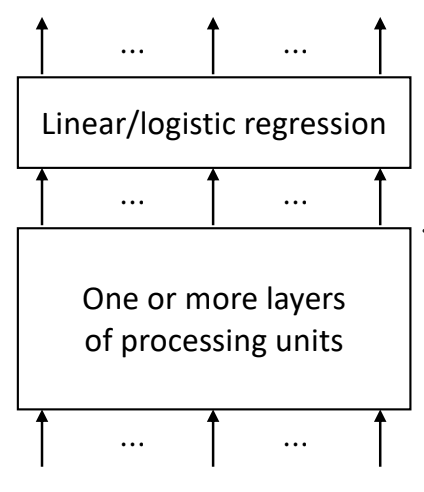
\includegraphics[scale=0.5]{img/FNN1.png}
\end{center}
\end{enumerate}
\subsection{Universal Approximation}
\begin{enumerate}
\item Analogous to \textbf{Turing machine} as a universal mathematical model of computation for today's digital computers, one would also like to know the universal mathematical model for feedforward neural networks.
\item An informal way of stating the universal approximation theorem (proved in the late 1980s) is that, a feedforward neural network with \textbf{sufficiently many sigmoid hidden units in only one layer} can approximate any well-behaved function to arbitrary precision. However, this theorem might have misled people not to put too much effort into exploring deeper neural networks.
\item Nevertheless, using more than one hidden layer may give a network that can approximate the same function using (exponentially) \textbf{fewer parameters} due to the high non-linearly that a deeper network can induce. This higher parameter efficiency also makes deeper networks much \textbf{faster to train}.
\item Deeper networks also mimic better the \textbf{hierarchical organization} of data in many real-world applications.
\end{enumerate}
\subsection{An illustrative example: a 3-layer network}
\begin{enumerate}
\item Each processing unit is shown as a circle. No processing is done in the input layer so no processing units are needed.
\begin{center}
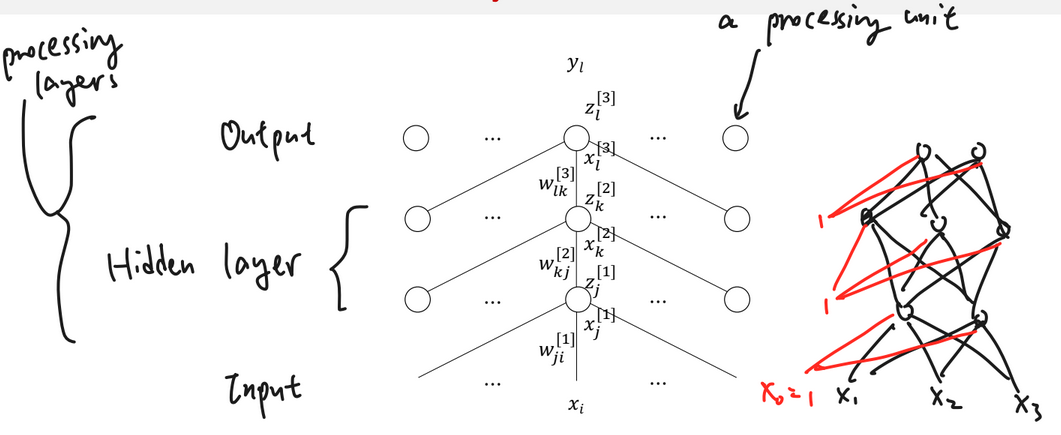
\includegraphics[scale=0.5]{img/FNN2.png}
\end{center}
\item There are \textbf{bias terms} for all the processing layers.
\item We consider here an illustrative example with 2 hidden layers to simply the notation. However, we still call it a 3-layer network as the output layer also count as a layer with processing units.
\item The superscripts, e.g., $[1], [2]$, refer to the corresponding network layers.
\item For each processing unit, 
\begin{enumerate}
\item its (summed) input is denoted by $x^{[*]}$;\\ e.g., $x^{[1]}_{j}$ means the input to $j$-th unit in the first hidden layer.
\item its output is denoted by $z^{[*]}$;\\ e.g., $z^{[1]}_{j}$ means the output from $j$-th unit in the first hidden layer.
\end{enumerate}
\item The input layer may also be denoted using the superscript $[0]$.
\end{enumerate}
\subsection{Activation Functions}
\begin{enumerate}
\item The function relating the input and output of a processing unit is called an activation function of the unit, e.g., $$z_{j}^{[1]} = g_{j}^{[1]}(x^{[1]}_j)$$
\item All the activation functions are \textbf{non-linear}, except for those in the output layer.
\item Note that if the activation functions of the 2 hidden layers are \textbf{linear}, then these 2 layers can be merge into one.
\begin{enumerate}
\item Input layer to first hidden layer: \\Input can be computed by $$x^{[1]}_j = \sum_{i} w^{[1]}_{ji} x_i$$ or in matrix form $$\mathbf{x}^{[1]} = \mathbf{W}^{[1]} \mathbf{x}^{[0]}$$; Output can be computed by $$z_{j}^{[1]} = g^{[1]}_{j} (x^{[1]}_{j})$$ or in matrix form $$\mathbf{z}^{[1]} = g^{[1]}(\mathbf{x}^{[1]})$$
\item First hidden layer to second hidden layer: \\Input can be computed by $$x^{[2]}_j = \sum_{j} w^{[2]}_{kj} z_j$$ or in matrix form $$\mathbf{x}^{[2]} = \mathbf{W}^{[2]} \mathbf{z}^{[1]}$$; Output can be computed by $$z_{k}^{[2]} = g^{[2]}_{k} (x^{[2]}_{k})$$ or in matrix form $$\mathbf{z}^{[2]} = g^{[2]}(\mathbf{x}^{[2]})$$
\item Second hidden layer to output layer: \\Input can be computed by $$x^{[3]}_l = \sum_{k} w^{[3]}_{lk} z_k$$ or in matrix form $$\mathbf{x}^{[3]} = \mathbf{W}^{[3]} \mathbf{z}^{[2]}$$; Output can be computed by $$z_{l}^{[3]} = g^{[3]}_{l} (x^{[3]}_{l})$$ or in matrix form $$\mathbf{z}^{[3]} = g^{[3]}(\mathbf{x}^{[3]})$$
\end{enumerate}
\item[] Sequentially, we can write \begin{align*}
\mathbf{z}^{[3]} &= g^{[3]}(\mathbf{x}^{[3]})\\
&=g^{[3]}(\mathbf{W}^{[3]} \mathbf{z}^{[2]})\\
&= g^{[3]}(\mathbf{W}^{[3]} g^{[2]}(\mathbf{x}^{[2]}))\\
&= g^{[3]}(\mathbf{W}^{[3]} g^{[2]}(\mathbf{W}^{[2]} \mathbf{z}^{[1]}))\\
&= g^{[3]}(\mathbf{W}^{[3]} g^{[2]}(\mathbf{W}^{[2]} g^{[1]}(\mathbf{x}^{[1]})))\\
&= g^{[3]}(\mathbf{W}^{[3]} g^{[2]}(\mathbf{W}^{[2]} g^{[1]}(\mathbf{W}^{[1]} \mathbf{x}^{[0]})))
\end{align*}
If $g^{[1]}$, $g^{[2]}$, and $g^{[3]}$ are linear, we can write $$\mathbf{z}^{[3]} = \mathbf{W}^{[3]}\mathbf{W}^{[2]} \mathbf{W}^{[1]} \mathbf{x}^{[0]} = \mathbf{W'} \mathbf{x}^{[0]}$$, that is, we can merge 3 layers in to one.
\item One exception is in an autoencoder in which a linear function may be used in the hidden units.
\item The logistic function for logistic regression can also seen as an activation function.
\end{enumerate}
\subsection{Loss Functions}
Recall these loss functions:
\begin{enumerate}
\item Squared loss function for regression problems
$$L(\mathbf{W}; \mathcal{S}) = \frac{1}{2} \sum_{q=1}^{N} \sum_{l} (z_{l} ^{[3](q)} - y_{l}^{(q)})^2 = \frac{1}{2} \sum_{q=1}^{N} \sum_{l} (x_{l} ^{[3](q)} - y_{l}^{(q)})^2 $$ The constant $\frac{1}{2}$ is introduced to simplify the subsequent derivation.
\item Cross-entropy loss function for classification problems
$$L(\mathbf{W}; \mathcal{S}) = -\sum_{q=1}^{N} \sum_{l} y^{(q)}_l \log z_{l}^{[3] (q)} = -\sum_{q=1}^{N} \sum_{l} y^{(q)}_l \log \texttt{softmax}(x^{[3] (q)}_l)$$
\end{enumerate}
\subsection{Back-propagation Learning Algorithm}
\begin{enumerate}
\item \textbf{Gradient descent} based on the gradients computed recursively in the backward direction starting from the output layer:
$$\Delta w^{[3]}_{lk} \propto - \pddx{L}{w_{lk}^{[3]}}, \Delta w^{[2]}_{kj} \propto - \pddx{L}{w_{kj}^{[2]}}, \Delta w^{[1]}_{ji} \propto - \pddx{L}{w_{ji}^{[1]}}$$
\item This recursive way of gradient computation for gradient descent is called the back-propagation (BP) learning algorithm.
\item Strictly speaking BP is not a recursive algorithm in the usual programming language sense. They share the same spirit though, e.g., computing $n!$ requires doing something (multiplying by $n$) to the result of $(n-1)!$.
\item More advanced gradient-based learning algorithms may also make use of the gradients computed this way.
\item Algorithm Sketch for (Batch) BP Learning
\begin{algorithm}
    \caption{Batch BP Learning}
    \begin{algorithmic}[1]
        \State Initialize variables
        \Repeat
        	\For {each training example $\mathbf{x}$} 		       		
        		\State predicted-output $\gets$ neural-network-output($\mathbf{x}$) \Comment{Forward propagation}
        		\State actual-output $\gets$ label($\mathbf{x}$)
        		\State Compute error terms at output units by a loss function  
        		\State
        		\State Compute weights changes for last layers of weights ($\Delta w^{[3]}$) \Comment{Backward propagation}
        		\State Compute weights changes for second layers of weights ($\Delta w^{[2]}$)
        		\State Compute weights changes for first layers of weights ($\Delta w^{[1]}$)
        	\EndFor
            \State Update network weights for all layers
        \Until{some stopping criterion is satisfied}
    \end{algorithmic}
\end{algorithm}
\item Gradients computations\\
We first let $$L^{(q)} = \begin{cases} 
\frac{1}{2} \sum_{l} (z_{l}^{[3](q)}-y_{l}^{(q)})^2 \text{ if regression}\\
- \sum_{l} y_{l}^{(q)} \log z_{l}^{[3](q)} \text{ if classification}
\end{cases}$$
\begin{enumerate}
\item Gradients of the last layer of weights $w_{lk}^{[3]}$
\begin{align*}
\pddx{L}{w_{lk}^{[3]}} &= \sum_{q=1}^{N} \pddx{L^{(q)}}{w^{[3]}_{lk}}\\
&= \sum_{q=1}^{N} \pddx{L^{(q)}}{x_{l}^{[3](q)}} \pddx{x^{[3](q)}}{w^{[3]}_{lk}}\\
&= -\sum_{q=1}^{N} \delta^{[3](q)} \pddx{x^{[3](q)}}{w^{[3]}_{lk}}
\end{align*}
So, to compute $\pddx{L}{w_{lk}^{[3]}}$, we need both $\delta^{[3](q)}$ and $\pddx{x^{[3](q)}}{w^{[3]}_{lk}}$
\begin{enumerate}
\item Compute $\delta^{[3](q)}$:
\begin{enumerate}
\item[](for regression)
\begin{align*}
\delta^{[3](q)} &= -\pddx{L^{(q)}}{x_{l}^{[3](q)}}\\
&= -\sum_{m} \pddx{L^{(q)}}{z_{m}^{[3](q)}} \pddx{z_{m}^{[3](q)}}{x_{l}^{[3](q)}}\\
&= - \pddx{L^{(q)}}{z_{l}^{[3](q)}} \pddx{z^{[3](q)}_l}{x^{[3](q)}_{l}}\\
&= y^{(q)}_{l} - z^{[3](q)}_{l}
\end{align*}
\item[] (for classification) 
\begin{align*}
\delta^{[3](q)} &= -\pddx{L^{(q)}}{x_{l}^{[3](q)}} \\
&= -\sum_{m} \pddx{L^{(q)}}{z_{m}^{[3](q)}} \pddx{z_{m}^{[3](q)}}{x_{l}^{[3](q)}}\\
&= \sum_{m} \frac{y_{m}^{(q)}}{z_{m}^{[3](q)}} z^{[3](q)}_{m} (\delta_{ml} - z_{l}^{[3](q)})\\
&= \sum_{m} y_{m}^{(q)} (\delta_{ml} - z_{l}^{[3](q)}) \\
&= y_{l}^{(q)} - z_{l}^{[3](q)}
\end{align*}
\textit{Remarks: the terms $\delta_l ^{[3](q)}$ can be regarded as the error terms computed at the output layer.}
\end{enumerate}
\item Compute $\pddx{x^{[3](q)}}{w^{[3]}_{lk}}$:
$$\pddx{x^{[3](q)}}{w^{[3]}_{lk}} = z_{k}^{[2](q)}$$
\end{enumerate}

\item Gradients of the second layer of weights $w_{kj}^{[2]}$
\begin{align*}
\pddx{L}{w_{kj}^{[2]}} &= \sum_{q=1}^{N} \pddx{L^{(q)}}{w_{kj}^{[2]}}\\
&= \sum_{q=1}^{N} \pddx{L^{(q)}}{x_k ^{[2](q)}}\pddx{x_k ^{[2](q)}}{w_{kj}^{[2]}}\\
&= - \sum_{q=1}^{N} \delta^{[2](q)}_k \pddx{x_k ^{[2](q)}}{w_{kj}^{[2]}}
\end{align*}, where \begin{align*}
\delta^{[2](q)}_k &= - \pddx{L^{(q)}}{x^{[2](q)}_k}\\
&= - \sum_{l} \pddx{L^{(q)}}{x^{[3](q)}_l} \pddx{x^{[3](q)}_l}{z^{[2](q)}_k} \pddx{z^{[2](q)}_k}{x^{[2](q)}_k}\\
&= \sum_{l} \delta^{[3](q)}_l w^{[3]}_{lk} g^{[2]'}_k (x^{[2](q)}_k)
\end{align*}\\ \textit{Remarks: the error terms $\delta_{k}^{[2](q)}$ of the second hidden layer are computed based on $\delta^{[3](q)}_l$}; and $$\pddx{x^{[2](q)}}{w^{[2]}_{kj}} = z_{j}^{[1](q)}$$

\item Gradients of the first layer of weights $w_{ji}^{[1]}$
\begin{align*}
\pddx{L}{w_{ji}^{[1]}} &= \sum_{q=1}^{N} \pddx{L^{(q)}}{w_{ji}^{[1]}}\\
&= \sum_{q=1}^{N} \pddx{L^{(q)}}{x_j ^{[1](q)}}\pddx{x_j ^{[1](q)}}{w_{ji}^{[1]}}\\
&= - \sum_{q=1}^{N} \delta^{[1](q)}_j \pddx{x_j ^{[1](q)}}{w_{ji}^{[1]}}
\end{align*}, where \begin{align*}
\delta^{[1](q)}_k &= - \pddx{L^{(q)}}{x^{[1](q)}_j}\\
&= - \sum_{l} \pddx{L^{(q)}}{x^{[2](q)}_k} \pddx{x^{[2](q)}_k}{z^{[1](q)}_j} \pddx{z^{[1](q)}_j}{x^{[1](q)}_j}\\
&= \sum_{k} \delta^{[2](q)}_k w^{[2]}_{kj} g^{[1]'}_j (x^{[1](q)}_j)
\end{align*}\\ \textit{Remarks: the error terms $\delta_{j}^{[1](q)}$ of the first hidden layer are computed based on $\delta^{[2](q)}_k$}; and $$\pddx{x^{[1](q)}}{w^{[1]}_{ji}} = x^{[1](q)}_i$$
\end{enumerate}
\item Weights Update Rules
\begin{enumerate}
\item Last layer: \begin{align*}
\delta_{l}^{[3](q)} &= y^{(q)}_{l} - z^{[3](q)}_l\\
\Delta w^{[3]}_{lk} &= -\eta \pddx{L}{w^{[3]}_{lk}} = \eta \sum_{q=1}^{N} \delta^{[3](q)}_{l} z^{[2](q)}_k
\end{align*}
\item Second layer: \begin{align*}
\delta_{k}^{[2](q)} &= \sum_{l} \delta^{[3](q)}_l w^{[3]}_{lk} g^{[2]'}_k (x^{[2](q)}_k)\\
\Delta w^{[2]}_{kj} &= -\eta \pddx{L}{w^{[2]}_{kj}} = \eta \sum_{q=1}^{N} \delta^{[2](q)}_k z^{[1](q)}_j
\end{align*}
\item First layer: \begin{align*}
\delta_{j}^{[1](q)} &= \sum_{k} \delta^{[2](q)}_k w^{[2]}_{kj} g^{[1]'}_j (x^{[1](q)}_j)\\
\Delta w^{[1]}_{ji} &= -\eta \pddx{L}{w^{[1]}_{ji}} = \eta \sum_{q=1}^{N} \delta^{[1](q)}_j x^{(q)}_i
\end{align*}
\end{enumerate}

\item Common Activation Functions
\begin{enumerate}
    \item Sigmoid $\sigma (x) = \frac{1}{1 + e^{-x}}$
    \item Hyperbolic tangent $\tanh(x) = \frac{e^x - e^{-x}}{e^x + e^{-x}}$
    \begin{center}
        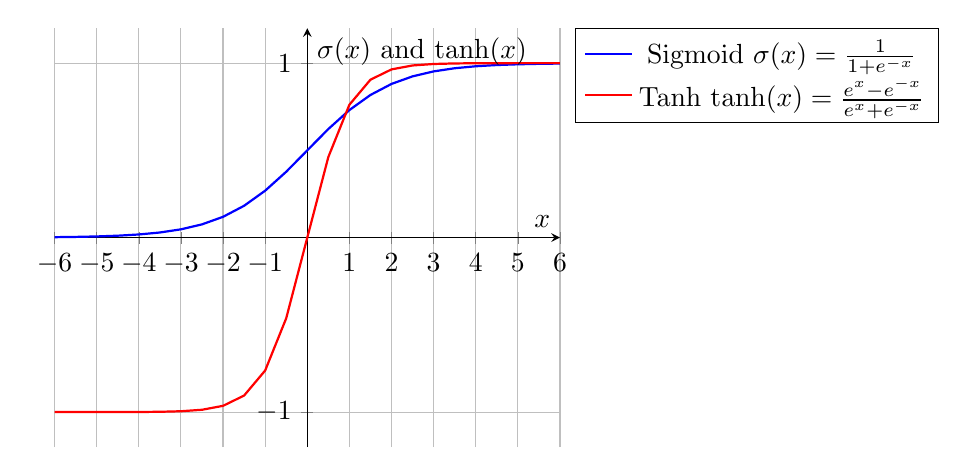
\begin{tikzpicture}
            \begin{axis}[
                axis lines = middle,
                xlabel = \(x\),
                ylabel = {\(\sigma(x)\) and \(\tanh(x)\)},
                xmin = -6, xmax = 6,
                ymin = -1.2, ymax = 1.2,
                xtick={-6,-5,...,6},
                ytick={-1,0,1},
                legend pos=outer north east,
                grid = both,
                domain=-6:6,
            ]
            % Sigmoid function
            \addplot[blue, thick] {1/(1 + exp(-x))};
            \addlegendentry{Sigmoid \(\sigma(x) = \frac{1}{1 + e^{-x}}\)}
        
            % Tanh function
            \addplot[red, thick] {tanh(x)};
            \addlegendentry{Tanh \(\tanh(x) = \frac{e^x - e^{-x}}{e^x + e^{-x}}\)}
            \end{axis}
        \end{tikzpicture}
    \end{center}
    \textit{Remarks:} 
    \begin{enumerate}
        \item Relationship between the two activation functions
        \begin{align*}
            \tanh (x) &= \frac{e^x - e^{-x}}{e^x + e^{-x}} \\
            &= 2 \cdot \sigma(2x) -1\\
            &= \frac{2}{1+e^{-2x}} -1
        \end{align*}
        \item Between these two activation functions, $\tanh$ should be a better choice for the hidden layers since it can take both positive and negative values (also zero) as its output for more comprehensive representation.
    \end{enumerate}
\end{enumerate}
\item Vanishing Gradient Problem\\
When we differentiate the activation functions $\sigma (x)$ and $\tanh (x)$, we get
\begin{align*}
    \sigma'(x) &= \frac{e^{-x}}{(1+e^{-x})^2}& \tanh'(x)&=2 \cdot \sigma'(2x)\\
    &= \frac{e^x}{(e^x +1)^2} &&= \frac{2e^{2x}}{(e^{2x}+1)^2}
\end{align*}
We can see that when $x$ is large in magnitude, both the gradients of $\sigma (x)$ and $\tanh (x)$ are very close to $0$. That is, their output does not chnage much when the input becomes very large in magnitude. We call them \emph{Saturating Activation Functions}.

If the activation function $g$ used in the neurons is saturating, the vanishing gradient problem may arise (especially when there are many hidden layers).
\begin{align*}
    \delta^{[2](q)}_k &= \sum_{l} \delta^{[3](q)}_{l} w^{[3]}_{lk} g^{[2]'}_{k} (x^{[2](q)}_{k})\\
    \delta^{[1](q)}_j &= \sum_{k} \delta^{[2](q)}_{k} w^{[2]}_{kj} g^{[1]'}_{j} (x^{[1](q)}_{j})
\end{align*}
The weight changes $\delta^{[2](q)}_k$ and $\delta^{[1](q)}_j$ will be very small, and thus the weight will not be updated probably. The techniques for overcomming the vanishing gradient problem in deep neural networks will be discussed in the next topic.

\item Stochastic Gradient Descent
\begin{enumerate}
    \item For feedforward neural network with one or more hidden layers, the loss function is no longer convex, i.e., local minima exist.
    \item While (batch) gradient descent computes the gradients by summing over all $N$ examples in the training set, Stochastic Gradient Descent (SGD) sums over a (usually much smaller) mini-batch of the trainign examples at a time.
    \item SGD can be regarded as a Stochastic Approximation of (batch) gradient descent with faster convergence.
    \item SGD is a more favorable alternative when the training set is large.
    \item SGD is also good at avoiding being trapped in a local minimum because SGD has more randomness than (batch) gradient descent, making SGD more likely to jump out of a local minimum.
\end{enumerate}

\item Regularization
\begin{enumerate}
    \item Regularized loss function based on $L_2$ regularization: $$L_{\lambda}(\mathbf{W}; \mathcal{S}) = L(\mathbf{W}; \mathcal{S}) + \frac{\lambda}{2} \sum_{w\text{ except bias terms}} w^2$$
    \item Weight update rule for $w$ (except the bias term) $$\Delta w = - \eta \pddx{L_{\lambda}}{w} = \eta \pddx{L}{w} - \eta \lambda w$$, where the second term is called the \emph{weight decay} term because it moves the weight towards zero.
\end{enumerate}

\item Momentum\\
We used it to stablise the SGD learning process.
\begin{enumerate}
    \item A \emph{momentum} term can be added to the weight update rule for $w$ to improve the speed of convergence $$\Delta w = - (1-\beta) \eta \pddx{L}{w} + \eta \Delta w^{\text{prev}}$$, where $L$ refers to the loss for a mini-batch, the momentum parameter $\beta$ is generally taken to be between 0.5 and 1 and $\Delta w^{\text{prev}}$ refers to the previous weight update.
    \begin{center}
        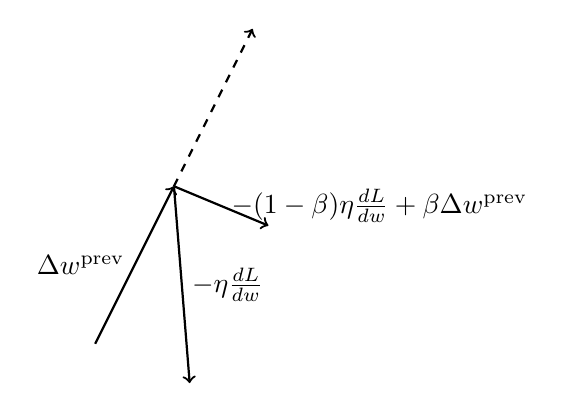
\begin{tikzpicture}[thick,->, scale=1]
            \coordinate (A) at (0, 0);
            \coordinate (B) at (1, 2);
            \coordinate (C) at (2, 4);
            \coordinate (D) at (1.2, -0.5);
            \coordinate (F) at (2.2, 1.5);
    
            \draw[->] (A) -- (B) node[midway, left] {\(\Delta w^{\text{prev}}\)};
            \draw[->] (B) -- (D) node[midway, right] {\(-\eta \frac{dL}{dw}\)};
            \draw[->] (B) -- (F) node[midway, right] {\(- (1 - \beta) \eta \frac{dL}{dw} + \beta \Delta w^{\text{prev}}\)};
            \draw[dashed, ->] (B) -- (C);
        \end{tikzpicture}
    \end{center}
    \item The momentum term is more crucial for SGD to make the learning process more stable by smoothing the weight changes over time.
    \item It has been shown mathematically that the momentum term plays a role similar to the \emph{mass} in damped harmonic oscillators by bringing the system closer to critical damping.
\end{enumerate}
\end{enumerate}

\section{Deep Neural networks}
\subsection{Challenges of trainign deep neural networks}
\begin{enumerate}
    \item The vanishing gradient problem makes the lower layers (i.e., the layers closer to the input layer) of a deep neural network very difficult to train, because the gradient of the often get smaller and smaller in magnitude as the BP algorithm progresses down to the lower layer.
    \item The many network weights in a deep neural network make it easy to overfit the training data.
    \item It would be extremely time consuming to train a large network especially when simple optimizers are used.
\end{enumerate}
\subsection{Non-saturating activation functions}
\begin{enumerate}
    \item Rectifier Linear Unit (ReLU) \\ ReLU is a processing unit that uses the rectifier $$g(x) =  \max(0, x) = \begin{cases} x & \text{ if } x \geq 0\\ 0 & \text{ otherwise} \end{cases}$$ as the activation function. ReLU alleviates the vanishing gradient problem because it does not saturate for positive input values.
    \begin{center}
        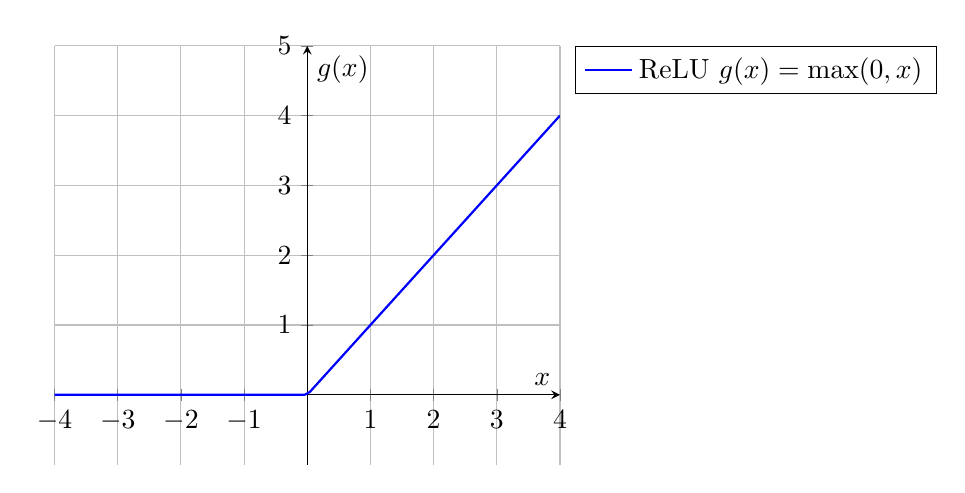
\begin{tikzpicture}
            \begin{axis}[
                axis lines = middle,
                xlabel = \(x\),
                ylabel = {\(g(x)\)},
                xmin = -4, xmax = 4,
                ymin = -1, ymax = 5,
                xtick={-4,-3,...,4},
                ytick={0,1,2,3,4,5},
                legend pos=outer north east,
                grid = both,
                domain=-4:4,
                samples=100,
            ]
            \addplot[blue, thick] {max(0,x)};
            \addlegendentry{ReLU \(g(x) = \max(0, x)\)}
            \end{axis}
        \end{tikzpicture}
    \end{center}
    \begin{enumerate}
        \item Another advantage of using the rectifier activation is that its derivative is easy to compute.
        \begin{align*}
            g(x) &= \begin{cases} x & \text{ if } x \geq 0\\ 0 & \text{ otherwise} \end{cases}& g'(x) &=\begin{cases} 1 & \text{ if } x \geq 0\\ 0 & \text{ otherwise} \end{cases}
        \end{align*}
        Meanwhile, computation of derivative of sigmoid function requires floating point computing.
        \item However, the vanishing gradient problem is not completely addressed because the gradient is $0$ for negative inpute values. When this happens, the output is $0$ and the gradient is $0$, making the \emph{dying ReLU} unlikely to come back to life again.
        \item Also, although the function is continous, it is not differentiable when the input is $0$. Nevertheless, this usually does not cause any problem in practice as we can use some programming tricks to solve this problem.
        \item A smooth approximation to the rectifier is the softplus function $$g(x) = \log(1+e^x)$$. Note that the derivative of softplus is the logistic function $$g'(x) = \frac{e^x}{1+e^{x}} = \frac{1}{1+e^{-x}}$$
        \begin{center}
            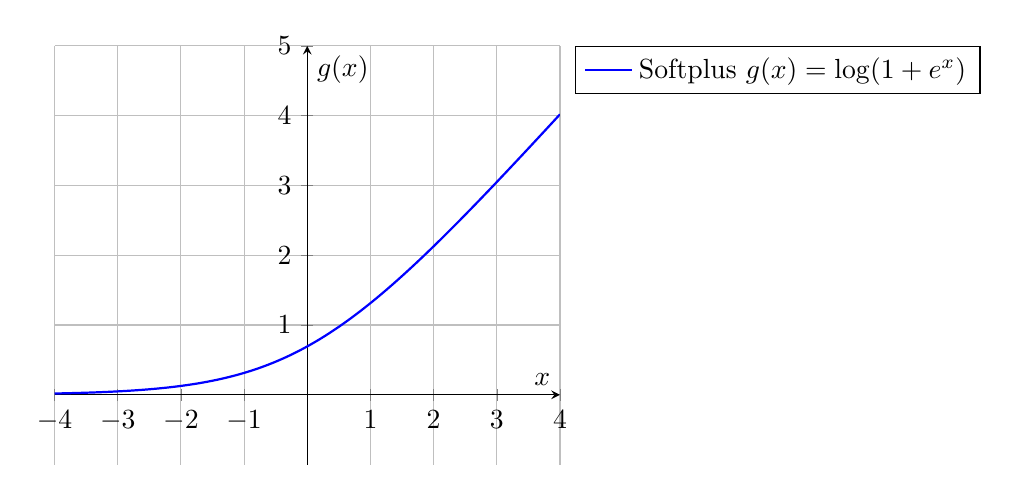
\begin{tikzpicture}
                \begin{axis}[
                    axis lines = middle,
                    xlabel = \(x\),
                    ylabel = {\(g(x)\)},
                    xmin = -4, xmax = 4,
                    ymin = -1, ymax = 5,
                    xtick={-4,-3,...,4},
                    ytick={0,1,2,3,4,5},
                    legend pos=outer north east,
                    grid = both,
                    domain=-4:4,
                    samples=100,
                ]
                \addplot[blue, thick] {ln(1 + exp(x))};
                \addlegendentry{Softplus \(g(x) = \log(1 + e^x)\)}
                \end{axis}
            \end{tikzpicture}
        \end{center}
    \end{enumerate}
    \item Leaky ReLU\\ Leaky ReLU improves ReLU by allowing a small positive gradient for negative input values (e.g., $\alpha =  0.01$). 
    \begin{align*}
        g(x) &= \begin{cases} x & \text{ if } x \geq 0\\ \alpha x & \text{ otherwise} \end{cases}& g'(x) &=\begin{cases} 1 & \text{ if } x \geq 0\\ \alpha & \text{ otherwise} \end{cases}
    \end{align*}
    \begin{center}
        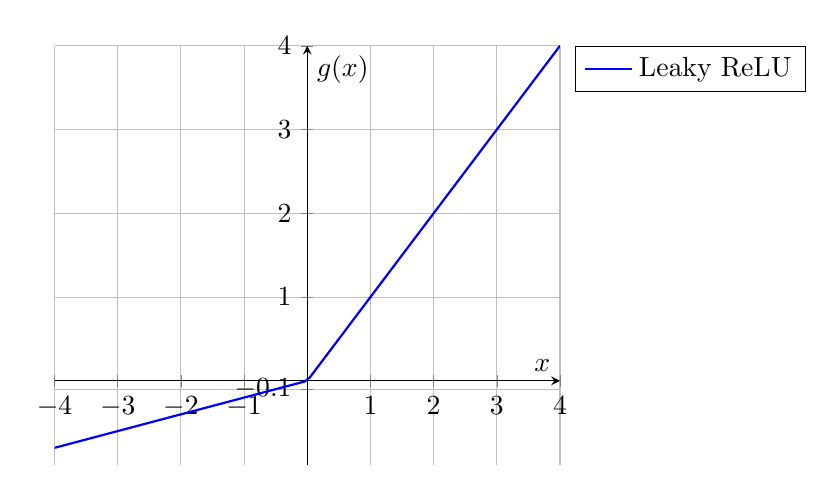
\begin{tikzpicture}
            \begin{axis}[
                axis lines = middle,
                xlabel = \(x\),
                ylabel = {\(g(x)\)},
                xmin = -4, xmax = 4,
                ymin = -1, ymax = 4,
                xtick={-4,-3,...,4},
                ytick={-0.1,0,1,2,3,4,5},
                legend pos=outer north east,
                grid = both,
                domain=-4:4,
                samples=100,
            ]
            \addplot[blue, thick] {x >= 0 ? x : 0.2 * x};
            \addlegendentry{Leaky ReLU}
            \end{axis}
        \end{tikzpicture}
    \end{center}

    \item Exponential Linear Unit (ELU)\\ Exponential linear unit (ELU) has the following activation function: $$g(x) = \begin{cases} x& \text{ if }x \geq 0 \\ \alpha (e^x -1) & \text{ otherwise}\end{cases}$$, where $\alpha > 0$ is a hyperparameter (e.g., initialised to $1$). Note that the derivative of ELU is $$g'(x) = \begin{cases} 1& \text{ if }x \geq 0 \\ \alpha e^x = g(x) + \alpha & \text{ otherwise}\end{cases}$$. 
    \begin{enumerate}
        \item An advantage of ELU is that its mean activation value is close to $0$, which can be proved to enable faster learning. Since the softplus function always gives a positive value, it is not as good as ELU.
        \item Unlike ReLu and its variants, the activation function of ELU is \emph{smooth everywhere}, include around $x = 0$, which speed up gradient descent because it does not bounce as much left and right of $x = 0$.
        \item The main drawback of the ELU activation funciton is that it is slower to compute than ReLU and its variants due to its use of exponential function. This is not too much of a problem during training because the slower computation is compensated by the faster convergence, but testing it will be considerably slower than ReLU.
        \item There is a variant of ELU, called scaled ELU (SELU), which has an additional hyperparameter $\lambda$ to achieve internal normalization. $$\text{SELU} = \lambda \text{ELU}(x) = \begin{cases} \lambda x& \text{ if }x \geq 0 \\ \lambda \alpha (e^x -1) & \text{ otherwise}\end{cases}$$
    \end{enumerate}
\end{enumerate}

\subsection{Choosing activation functions}
\begin{enumerate}
    \item If runtime performance is NOT a concern, in general the relative performance of different choice is: ELU $>$ leaky ReLU (and its variants) $>$ ReLU $>$ $\tanh$ $>$ sigmoid
    \item If runtime is an important factor to consider, leaky ReLU will be a better choice than ELU.
    \item The hyperparameter in leaky ReLU and ELU may be learned to further boost the performance if the training set is sufficiently large (or else overfitting may occur). 
\end{enumerate}

\subsection{Weight initialization}
\begin{enumerate}
    \item Observations (which are consequences of using non-saturating activation function such as ReLU)
        \begin{enumerate}
            \item If the weights in a network start too small, then the signal shrinks as it passes through each layer until it is too tiny to be useful. 
            \item If the weights in a network start too large, then the signal grows as it passes through each layer until it is too massive to be useful. 
        \end{enumerate}
    \item Xavier Initialisation 
    \begin{enumerate}
        \item The weight intialization strategy called Xavier initialization (named after the author's first name) makes sure the weights in a reasonable range of values so that the signals can reach deep into network. 
        \item The main idea is to let the distribution governing the intialization of weights depend on the number of input connections and the number of output connections for the layer whose weights are being initialised. 
        \item Let $\begin{cases}n_{\text{in}} &:= \text{number of input connections in a layer}\\
        n_{\text{out}} &:= \text{number of output connections in a layer} \end{cases} $, the weights may be initialised randomly using a normal distribution $$\mathcal{N}(0, \dfrac{2}{n_{\text{in}} + n_{\text{out}}})$$ or a uniform distribution $$\mathcal{U}(- \sqrt{\dfrac{6}{n_{\text{in}} + n_{\text{out}}}}, +\sqrt{\dfrac{6}{n_{\text{in}} + n_{\text{out}}}})$$.
    \end{enumerate}
    \item He Initialisation
    \begin{enumerate}
        \item The He initialisation (named after the author's last name), also called Kaiming initialisation (named after the author's first name), is for ReLU and its variants, including ELU.
        \item Similar to Xavier Initialisation, the weights may be intialsed using a normal distribution $$\mathcal{N}(0, \dfrac{4}{n_{\text{in}} + n_{\text{out}}})$$ or a uniform distribution $$\mathcal{U}(- \sqrt{\dfrac{12}{n_{\text{in}} + n_{\text{out}}}}, +\sqrt{\dfrac{12}{n_{\text{in}} + n_{\text{out}}}})$$.
    \end{enumerate}
\end{enumerate}
\subsection{Batch Normalisation}
\begin{enumerate}
    \item Internal Covariate Shift
    \begin{enumerate}
        \item Although using a carefully designed weight initialisation strategy along with a non-saturating activation function such as leacky ReLU or ELU can significantly alleviate the vanishing/ exploring gradient problem at the beginning of training, this problem may still arise later during training.
        \item The internal covariate shift problem refers that the distribution of the inputs of each layer changes during training  as the network weights of the previous layers change.
    \end{enumerate}
    \item Overviews of batch normalisation\\Batch normalisation is a technique for addressing the vanishing/ exploding gradient problem by addressing the more general internal covariate shift problem.
    \begin{enumerate}
        \item In a way, batch normalisation can be seen as extending the idea of normalising the raw input to the upper layers of the network
        \item Before applying the activation function of each layer, the mean and variance of the inputs over the current mini-batch are evaluated to zero-center and normalise the inputs by the evaluated variance. (Hence, the name "batch" normalisation).
        \item Two new parameters $\gamma, \beta$, one for scaling and the other for shifting, are learnt for each layer to restore its representation power.
        \item Unlike normalising the input which are done for the whole batch, batch normalisation does it for each mini-batch separately.
        \item While batch normalisation is generally quite effective, the true reason why and how it works is still not fully understood.
    \end{enumerate}
    \item Transform with Learning Parameters
    \begin{enumerate}
        \item Batch normalising transform applied over a mini-batch
        \begin{algorithm}
            \caption{Batch Normalising Transform}
            \begin{algorithmic}[1]
                \State \textbf{Input}: Values of $x$ over a mini-batch: $\mathcal{B} = \{x_{1 \cdots m}\}$
                \State \textbf{Output}: $\{y_i = \text{BN}_{\gamma, \beta}(x_i)\}$\\
                $\mu_{\mathcal{B}} \gets \dfrac{1}{m} \sum_{i=1}^{m} x_i$ \Comment{mini-batch mean}\\
                $\sigma_{\mathcal{B}}^2 \gets \dfrac{1}{m} \sum_{i=1}^{m} (x_i - \mu_{\mathcal{B}})^2$ \Comment{mini-batch variance}\\
                $\hat{x}_i \gets \dfrac{x_i - \mu_{\mathcal{B}}}{\sqrt{\sigma_{\mathcal{B}}^2 + \epsilon}}$ \Comment{normalise}\\
                $y_i \gets \gamma \hat{x}_i + \beta \equiv \text{BN}_{\gamma, \beta}(x_i)$ \Comment{scale and shift}
            \end{algorithmic}
        \end{algorithm}
        \item The transform can be implemented by introducing an additional layer with learnable parameters $\gamma, \beta$.
        \item With batch normalisation, the vanishing gradient problem can be significantly reduced even when saturating activation functions such as the sigmoid and hyperbolic tangent functions are used without relying on carefully designed weight initialisation and regularisation.
    \end{enumerate}
    \item Batch normalisation during prediction
    \begin{enumerate}
        \item Like dropout, batch normalisation has different computation results in training and prediction modes.
        \item During training, normalisation is based on the mini-batch statistics.
        \item During prediction, normalisation is based on the dataset statistics (i.e., the whole dataset).
    \end{enumerate}
\end{enumerate}
\subsection{Dropout}
\begin{enumerate}
    \item Dropout is a regularisation technique to prevent overfitting.
    \item At each training step, each hidden unit or input has a probability $p$ of being temporarily dropped out (i.e., ignored during this training step, but it may become active again during the next step). 
    \item The hyperparameter $p$, called the dropout rate, is typically set to $0.5$ (but other values are also possible, even with different values for different layers). Sometimes it is more convenient to refer to the keep probability with is equal to $1-p$. 
    \item In general, a higher dropout rate is used if more serious overfitting is observed and for layers with more units (and hence more parameters to estimate).
    \item Dropout is \emph{only applied during training} but not during testing.
    \item Dropout can also be applied to connections (i.e., weights), but we will focus on dropping out units here.
    \item Like L1/ L2 regularisation, dropout is only applied to the non-bias units.
    \item Justifications of dropout
    \begin{enumerate}
        \item Since hidden units and inputs are dropped out randomly, the network need to learn to be more robust (i.e., less sensitive to slight changes in the inputs) by replying on more incoming units or inputs rather than just a few, effective spreading out the weights to more units.
        \item An alternative way is to view dropout as \emph{emsemble learning}, in that each training step "generates" one of $2^{N}$ possible networks, where $N$ is the total number of droppable units or inputs, and trains the network on one example from the training set. The resulting neural network is essentially an emsemble of a large number of smaller networks.
    \end{enumerate}
    \item Since dropout is not applied during testing, a hidden unit will on average be connected to $\dfrac{1}{1-p}$ times as many inputs as it was during training. There are two alternative methods to deal with this problem.
    \begin{enumerate}
        \item Multiply the input weights of each unit by the keep probability $1-p$ after training.
        \item (Inverted dropout) Divide the output of each unit by the keep probability during training. 
    \end{enumerate}
    Strictly speaking, these two methods are not equivalent but they both work well. Specifically, nothing needs to be done during testing and hence inference will not be slowed down.
\end{enumerate}
\subsection{Data Augmentation}
\begin{enumerate}
    \item Overfitting can be reduced by having more training data, but it is not always possible to get more labelled training examples. 
    \item Data augmentation is a regularisation technique that generates new, synthetic training instances from existing ones to increase the size of the training set effectively.
    \item Data augmentation aims to explicitly let the model know the allowed invariances.
    \item Instead of wasting storage space and network bandwidth, it is preferable to generate new training instances \emph{on the fly} during training.
    \item Example: Image Data
    \begin{enumerate}
        \item Some commonly used operations:
    \begin{enumerate}
        \item Translation, rotation, or rotation by various amounts
        \item Lighting with varous contrasts
        \item Cropping 
        \item Flipping horizontally (but note that it is not suitable for some image-based applications such as character recognition).
    \end{enumerate}
    \item Some deep learning frameworks such as \texttt{TensorFlow} provide image manipulation operations for generating new training instances efficiently on the fly.
    \item Some generative models (such as GAN) and generative AI tools may also be used for data augmentation.
    \end{enumerate}
\end{enumerate}
\subsection{Optimizers}
\begin{enumerate}
    \item AdaGrad
    \begin{enumerate}
        \item Recall the ordinary Stochastic Gradient Descent (SGD): $$\mathbf{w} \gets \mathbf{w} - \eta \nabla_{\mathbf{w}} L$$, where $\nabla$ denotes the vector differential operator. 
        \item AdaGrad improves SGD using an adaptive learning rate which decays faster for steeper dimensions.
        \begin{align*}
            \mathbf{s} &\gets \mathbf{s} + \nabla_{\mathbf{w}} L \circ \nabla_{\mathbf{w}} L\\
            \mathbf{w} &\gets \mathbf{w} - \eta \nabla_{\mathbf{w}} L \oslash \sqrt{\mathbf{s + \epsilon}}
        \end{align*}, where $\circ$ denotes the Hadamard product (a.k.a. elementwise multiplication), $\oslash$ denotes the Hadamard division (a.k.a. elementwise division), and $\mathbf{\epsilon}$ is a smoothing term with a small value (e.g., $10^{-10}$) for all dimensions to avoid division by $0$.
        \item The first step of AdaGrad accumulates the square of the gradients into vector $\mathbf{s}$: a dimension of $\mathbf{s}$ will become larger and larger if the loss function is steep along that dimension.
        \item The second step is similar to SGD except that there is a scaling factor $\sqrt{\mathbf{s + \epsilon}}$: a dimension will decay its learning rate faster if the loss function is steep along that dimension. 
        \item With the adaptive learning rate (without requiring manual training), AdaGrad helps point the result updates more directly towards the global optimum.
        \item Although AdaGrad performs well for simple quadratic problems, it often stops too early before reaching the global optimum when used for training neural networks.
    \end{enumerate}
    \item RMSProp
    \begin{enumerate}
        \item To overcome the problem of AdaGrad which decays too fast, RMSProp does not accumulate all the gradient from the beginning but only from the recent iterations by introducing exponential decay in the first step. 
        \begin{align*}
            \mathbf{s} &\gets \beta \mathbf{s} + (1-\beta) \nabla_{\mathbf{w}} L \circ \nabla_{\mathbf{w}} L\\
            \mathbf{w} &\gets \mathbf{w} - \eta \nabla_{\mathbf{w}} L \oslash \sqrt{\mathbf{s + \epsilon}}
        \end{align*}, where the decay rate $\beta$ is typically set to $0.9$.
        \item If we explicitly add a time step as subscript and use $\mathbf{g}$ to denote $\nabla_{\mathbf{w}} L \circ \nabla_{\mathbf{w}} L$, the first step of RMSProp can be expressed as the recurrence relation $\mathbf{s}_{t} = \beta \mathbf{s}_{t-1} + (1 - \beta) \mathbf{g}_{t}$. Iterating this recurrence yields the following: $$\mathbf{s}_{t} = \beta^t + (1-\beta)(\beta^{t -1} \mathbf{g}_1 + \beta^{t -2} \mathbf{g}_2 + \cdots + \beta \mathbf{g}_{t-1} + \mathbf{g}_t) = \beta^t + \sum_{i=1}^{t} \beta^{t-i} \mathbf{g}_{i}$$
    \end{enumerate}
    \item Adam (adaptive moment estimation)
    \begin{enumerate}
        \item Adam combines the idead of momentum and RMSProp.
        \begin{enumerate}
            \item Like momentum, Adam keeps track of an exponential decaying average of the past gradients.
            \item Like RMSProp, it keeps track of an exponential decaying average of the past squared gradients.
        \end{enumerate}
        \begin{align*}
            \mathbf{\Delta w} &\gets \beta_1 \mathbf{\Delta w} - (1-\beta_1 \mathbf{\nabla_{w} L})\\
            \mathbf{s} &\gets \beta_2 \mathbf{s} + (1-\beta_2) \nabla_{\mathbf{w}} L \circ \nabla_{\mathbf{w}} L\\
            \mathbf{\Delta w} &\gets \dfrac{\mathbf{\Delta w}}{1 - \beta_1} & \mathbf{s} &\gets \dfrac{\mathbf{s}}{1 - \beta_2}\\
            \mathbf{w} &\gets \mathbf{w} + \eta \mathbf{\Delta w} \oslash \sqrt{\mathbf{s + \epsilon}}
        \end{align*}, where $t$ is the iteration number. The third step is for bias correction because the running averages are initialized to $0$.
        
    \end{enumerate}
    \item[] \emph{Remarks}: \begin{enumerate}
        \item Although Adam generally works well and is faster than other methods, a study showed that adaptive optimization methods including AdaGrad, RMSProp and Adam can give solutions that generalize poorly on some data sets.
        \item So there is no single method that is always the best.
    \end{enumerate}
\end{enumerate}
\end{document}